\documentclass[a4paper,11pt,oneside]{article}
\usepackage[T1]{fontenc}
\usepackage[utf8x]{inputenc}
\usepackage{lmodern,textcomp}
\usepackage[document]{ragged2e}
\usepackage{longtable}
\usepackage[english,main=french]{babel}
\usepackage[dvipsnames]{xcolor}

\usepackage[calc,useregional]{datetime2}
\usepackage{datenumber}
\usepackage{calc}
\newcounter{datetoday}
\newcounter{diffyears}
\newcounter{diffmonths}
\newcounter{diffdays}
\newcommand{\difftoday}[3]{%
      \setmydatenumber{datetoday}{\the\year}{\the\month}{\the\day}%
      \setmydatenumber{diffdays}{#1}{#2}{#3}%
      \addtocounter{diffdays}{-\thedatetoday}%
      \ifnum\value{diffdays}<0
        \setcounter{diffdays}{-\value{diffdays}}%
      \fi
      \setcounter{diffyears}{\value{diffdays}/365}%
      \setcounter{diffdays}{\value{diffdays}-365*\value{diffyears}}%
      \setcounter{diffmonths}{\value{diffdays}/30}%
      \setcounter{diffdays}{\value{diffdays}-30*\value{diffmonths}}%
      \ifnum\value{diffyears}=0
      \else
        \ifnum\value{diffyears}>1
            \thediffyears\space ans
        \else
            \thediffyears\space an
        \fi
      \fi
      \ifnum\value{diffmonths}=0
        1 mois
      \else
        \thediffmonths\space mois
      \fi
}

\newcommand{\fakesection}[1]{
  \par\refstepcounter{section}
  \sectionmark{#1}
  \addcontentsline{toc}{section}{#1}
}

\usepackage{advdate}
\usepackage{setspace}
\usepackage{hyperref}
\usepackage{url}
\hypersetup{colorlinks=true,linkcolor=RoyalBlue,urlcolor=RoyalBlue,citecolor=RoyalBlue,anchorcolor=RoyalBlue}
\urlstyle{same}
\usepackage{graphicx}
\usepackage[export]{adjustbox}
\usepackage{colortbl}

\usepackage[left=2cm,right=2cm,bottom=2cm,top=1.5cm,foot=0.5cm]{geometry}

\usepackage{lastpage}
\usepackage{fancyhdr}
\fancypagestyle{plain}{\fancyhead{}\renewcommand{\headrule}{}}
\pagestyle{plain}
\fancyhead{}
\renewcommand{\headrulewidth}{0pt}
\fancyfoot{}
\fancyfoot[L]{\small {\color{gray}Stéphane Ghozzi $\cdot$ Curriculum vitæ au \today}} 
\fancyfoot[R]{\small {\color{gray}page\ \thepage\ sur \pageref*{LastPage}}}
\pagenumbering{arabic}

\setcounter{secnumdepth}{0}
\usepackage{tocloft}
\renewcommand{\cftsecleader}{\cftdotfill{\cftsecdotsep}}
\renewcommand\cftsecdotsep{\cftdot}

\hyphenation{di-sease tra-vel-ling ana-ly-ses rea-lize vi-sua-li-za-tion a-na-ly-zing}

\usepackage{cite}

\begin{document}
\selectlanguage{french}

\noindent\begin{minipage}{0.7\linewidth}
   \LARGE
   \noindent\textbf{Stéphane Ghozzi}

   \normalsize
   \vspace{1.5em}
   \noindent Chercheur intéressé par le soutien, à travers analyses et visualisations interactives, de la préparation et la réponse en santé publique : application et évaluation d'approches d'apprentissage machine, développement et déploiement de tableaux de bord interactifs. Parcours de physique théorique fondamentale vers la biophysique et maintenant l'épidémiologie de maladies infectieuses. Adore assembler des équipes pluridisciplinaires, confortable en tant qu'analyste et développeur indépendant.
\end{minipage}
\begin{minipage}{0.3\linewidth}
   \begin{center}
      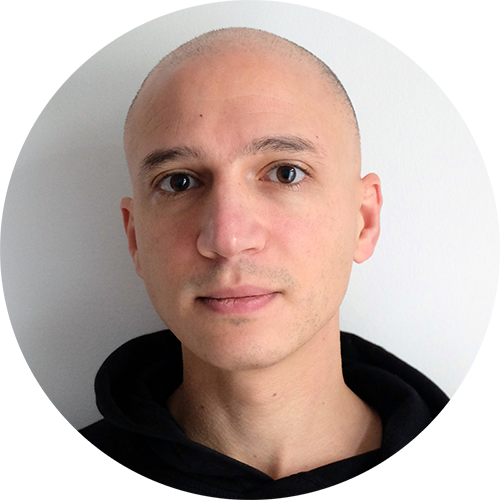
\includegraphics[width=0.55\textwidth,right]{GHOZZI-Stephane-portrait-2020-cropped-circle-nobackground-lr.png}
   \end{center}
\end{minipage} 

\vspace{1em}

\href{https://orcid.org/0000-0002-3911-9573}{orcid.org/0000-0002-3911-9573} $\cdot$ \href{https://gitlab.com/stephaneghozzi}{gitlab.com/stephaneghozzi} $\cdot$
\href{https://twitter.com/stephaneghozzi}{twitter.com/stephaneghozzi} $\cdot$\\ \href{https://www.linkedin.com/in/stephaneghozzi}{linkedin.com/in/stephaneghozzi} $\cdot$ \href{https://scholar.google.com/citations?user=uGVLwREAAAAJ}{scholar.google.com/citations?user=uGVLwREAAAAJ} $\cdot$ \\
\href{https://www.researchgate.net/profile/Stephane\_Ghozzi}{researchgate.net/profile/Stephane\_Ghozzi}

\vspace{1em}

\noindent {\color{gray}\hrule} 

\vspace{1em}

\noindent \begin{longtable}{@{}p{3.1cm}@{}@{}p{13.9cm}@{}}
   \Large{Expérience} & \\
   & \\
   \textbf{Assistant de} & \textbf{Helmholtz-Zentrum für Infektionsforschung (HZI)} \\
   \textbf{recherche} & {\color{gray}\DTMdisplaydate{2020}{6}{1}{-1} -- présent $\cdot$ \difftoday{2020}{6}{1}} \\ 
   & {\color{gray} Braunschweig, Allemagne} \\
   & \href{https://www.helmholtz-hzi.de/en/research/research-topics/bacterial-and-viral-pathogens/epidemiology/our-research/}{helmholtz-hzi.de/en/research/research-topics/bacterial-and-viral-pathogens/epidemiology/our-research/} $\cdot$ \href{https://sormas.org}{sormas.org}\\ 
   & Scientifique senior, méthodes statistiques et outils pour la santé publique, dans le département d'Épidemiologie (groupe Krause). \\
   & \\
   & \begin{tabular}[t]{@{}!{\color{gray}\vrule}p{0.2cm}@{}p{13.3cm}@{}}
      & \textit{Surveillance Outbreak Response Management and Analysis System} (SORMAS): 
      Soutien automatisé à la prise de décision par les utilisateur$\cdot$rice$\cdot$s de SORMAS. Stratégies pour amener les calculs jusqu'aux données de façon à permettre des analyses poussées sans compromettre la protection des données. \\
      & \\
      & Effet du changement climatique sur la dynamique de maladies infectieuses : Modélisation statistique de l'impact à court et long termes des changements environnementaux et démographiques sur la dynamique de la maladie de Lyme an Allemagne. \\
      & \\
      & Apprentissage machine pour la sérologie multiplex.\\
      & \\
      & Gestion et organization : \\
      & $\cdot$ interlocuteur pour les thèmes de l'analyse et des processus automatisés ;\\
      & $\cdot$ soutien d'étudiant$\cdot$e$\cdot$s ; \\
      & $\cdot$ demandes de financement. \\
   \end{tabular} \\     
   & \\
   & \\   
   & \textbf{Robert-Koch Institut (RKI)} \\
   & {\color{gray}\DTMdisplaydate{2016}{4}{15}{-1} -- \DTMdisplaydate{2020}{5}{31}{-1} $\cdot$ 4 ans 2 mois}\\ 
   & {\color{gray}Berlin, Allemagne}\\
   & \href{https://www.rki.de/signale-project}{rki.de/signale-project} \\
   & Apprentissage machine, informatique, statistique et visualisation, équipe Signale, Département d'Épidémiologie des Maladies infectieuses. \\
   & \\
   & \begin{tabular}[t]{@{}!{\color{gray}\vrule}p{0.2cm}@{}p{13.3cm}@{}}
      & Recherche et développement : \\
      & $\cdot$ développement d'algorithmes de détection d'épidémies et modélisation de dynamique d'infection ; \\
      & $\cdot$ évaluation de performance et optimisation de paramètres des algorithmes ; \\
      & $\cdot$ traitement automatique du langage naturel d'articles en ligne pour soutenir la surveillance international de maladies infectieuses ; \\
      & $\cdot$ visualisations interactives pour les professionnel$\cdot$le$\cdot$s des résultats et autres données. \\
      & \\
      & Gestion et organisation : \\
      & $\cdot$ porte-parole de l'équipe (quatre scientifiques des données, deux développeurs web, en moyenne deux étuditant$\cdot$e$\cdot$s en Master) ; \\
      & $\cdot$ coordination du \textit{Topic Group Outbreaks} du \textit{Focus Group AI for Health} de l'UIT et de l'OMS: \href{https://www.itu.int/en/ITU-T/focusgroups/ai4h/Pages/tg.aspx}{itu.int/en/ITU-T/focusgroups/ai4h/Pages/tg.aspx} \\
      & $\cdot$ encadrement de thèses de Master ; \\
      & $\cdot$ organisation de workshops et hackathons ; \\
      & $\cdot$ demandes de financement. \\
   \end{tabular} \\
   & \\
   & \\
   & \textbf{Organisation mondiale de la Santé (OMS)} \\
   & {\color{gray}\DTMdisplaydate{2019}{5}{1}{-1} -- \DTMdisplaydate{2019}{10}{31}{-1} $\cdot$ 6 mois} \\ 
   & {\color{gray}Geneva, Switzerland} \\
   & \href{https://www.who.int/eios}{who.int/eios} $\cdot$ \href{https://www.who.int/emergencies/outbreak-toolkit}{who.int/emergencies/outbreak-toolkit} \\
   & Apprentissage machine et développement d'application web pour le renseignement épidémiologique et les enquêtes d'épidémies d'origine inconnue.\\
   & \\
   & \begin{tabular}[t]{@{}!{\color{gray}\vrule}p{0.2cm}@{}p{13.3cm}@{}}
      & Dans les unités \textit{Detection, Verification and Risk Assessment} (DVA) et \textit{Health Operations Monitoring and Data Collection} (MDC) du département \textit{Health Emergency Information and Risk Assessment} (HIM) au sein du programme \textit{WHO Health Emergencies} (WHE). \\
   \end{tabular} \\
   & \\
   & \\
   \textbf{Artiste} & \textbf{indépendant} \\
   \textbf{plasticien} & {\color{gray}\DTMdisplaydate{2012}{3}{1}{-1} -- \DTMdisplaydate{2016}{4}{14}{-1} $\cdot$ 4 ans 1 mois} \\ 
   & {\color{gray}Berlin, Allemagne} \\
   & \href{http://www.stephaneghozzi.com}{stephaneghozzi.com} \\
   & Dessin, animation générative, photographie, vidéo, animation 3d. \\
   & \\   
   & \begin{tabular}[t]{@{}!{\color{gray}\vrule}p{0.2cm}@{}p{13.3cm}@{}}   
      & Sélection de projets et coopérations : \\
      & $\cdot$ 2014 : vidéos montrées dans le festival \textit{backup}, E-Werk, Weimar ; \\
      & $\cdot$ 2005 : douze illustrations pour \textit{Trace.project}, un album-compilation de musique électronique originale ; \\
      & $\cdot$ 2005 : vidéographie pour l'œuvre de dance \textit{Entre-Deux} de Mirjam Fruttiger, Paris and Rome (dont un séjour d'une semaine à la Villa Médicis); \\
      & $\cdot$ 2004 : vidéographie sur le documentaire \textit{Manchay Tiempo} de Florence Blum et María Pía Medina-Luna (tournage de quatre semaines au Pérou); \\
      & $\cdot$ 2002 : dessins et photographies publiés dans la revue \textit{R de réel}. \\
   \end{tabular} \\   
   & \\
   & \\
   \textbf{Chercheur} & \textbf{Institut für Theoretische Physik (THP), Universität zu Köln}\\
   \textbf{postdoctorant} & {\color{gray}\DTMdisplaydate{2010}{3}{1}{-1} -- \DTMdisplaydate{2012}{2}{29}{-1} $\cdot$ 2 ans}\\
   & {\color{gray}Cologne, Allemagne} \\
   & \url{www.thp.uni-koeln.de/~lassig} \\
   & Modèles statistiques et mécanistiques d'évolution biologique, dans le groupe Lässig. \\
   & \\
   & \begin{tabular}[t]{@{}!{\color{gray}\vrule}p{0.2cm}@{}p{13.3cm}@{}}
      & Modèle mathématique et analyse de la croissance et expression génétique bactériennes, interprétation de résultats expérimentaux. \\
      & \\
      & Signatures de sélection dans les séquences ADN et comparaison avec modèles de génétique des populations : \\
      & $\cdot$ évolution à long terme de virus de la grippe ; \\
      & $\cdot$ motifs de sites de fixation de facteurs de transcription chez la levure.\\
      & \\
      & Signatures de co-évolution dans les séquences de protéines. \\
   \end{tabular} \\   
   & \\   
   & \\   
   \textbf{Assistant} & \textbf{Universität zu Köln} \\
   \textbf{enseignement} & {\color{gray}\DTMdisplaydate{2010}{9}{1}{-1} -- \DTMdisplaydate{2012}{1}{30}{-1} $\cdot$ 1 an 5 mois} \\
   & {\color{gray}Cologne, Allemagne} \\   
   & Mathématiques et physique statistique pour étudiant$\cdot$e$\cdot$s en Bachelor.\\
   & \\
   & \textbf{UPMC Sorbonne Universités} \\
   & {\color{gray}\DTMdisplaydate{2005}{10}{1}{-1} -- \DTMdisplaydate{2009}{8}{31}{-1} $\cdot$ 3 ans 11 mois} \\
   & {\color{gray}Paris, France} \\
   & Thermodynamique, optique et ondes, méthodes mathématiques pour étudiants en Bachelor.\\
   & \\   
   & \\   
   \textbf{Doctorant} & \textbf{Laboratoire de Physique Statistique (LPS), École normale supérieure} \\
   & {\color{gray}\DTMdisplaydate{2005}{9}{1}{-1} -- \DTMdisplaydate{2009}{12}{31}{-1} $\cdot$ 4 ans 4 mois} \\
   & {\color{gray}Paris, France} \\
   & \href{http://www.labos.upmc.fr/ljp/?article7}{www.labos.upmc.fr/ljp/?article7} $\cdot$ \href{http://www.lps.ens.fr/?lang=en}{www.lps.ens.fr} \\
   & Biophysique théorique et expérimentale, dans le groupe Chatenay : Dynamique de réseaux de régulation génétique\\
   & \\
   & \begin{tabular}[t]{@{}!{\color{gray}\vrule}p{0.2cm}@{}p{13.3cm}@{}}
      & Titulaire d'une bourse de 60 k€ pour financer le projet expérimental (sur 3 ans, utilisé pour acheter du matériel et des consommables) : programme \flqq{} Interface physique, biologie et chimie : soutien à la prise de risque 2007-2009 \frqq{} du CNRS. \\
      & \\
      & Séries temporelles de niveaux d'expression génétique, par microscopie de fluorescence, du réseau de décision lyse-lysogénie du bactériophage Lambda : \\
      & $\cdot$ biologie moléculaire (extraction de gènes viraux, insertion de gènes codant pour des protéines fluorescentes, modification de génome bactérien) ; \\
      & $\cdot$ microbiologie (cultures bactériennes et virales) ; \\
      & $\cdot$ automatisation et microscopie de fluorescence ; \\
      & $\cdot$ analyse d'images. \\   
      & \\
      & Analyse mathématique de statistiques de bruits dans l'expression génétique bactérienne.\\
      & \\
      & Simulation informatiques de dynamiques et d'évolution de réseaux de régulation génétique.
   \end{tabular} \\
   & \\
   & \\   
   \textbf{Volontariat} & \textbf{Celsius} \\
   \textbf{Membre} & {\color{gray}\DTMdisplaydate{2007}{8}{1}{-1} -- \DTMdisplaydate{2009}{8}{31}{-1} $\cdot$ 2 ans 1 mois} \\
   \textbf{fondateur} & {\color{gray}Paris, France} \\
   & Celsius était un groupe de réflexion qui avait pour but de développer le projet européen.\\
   & \\   
   & \begin{tabular}[t]{@{}!{\color{gray}\vrule}p{0.2cm}@{}p{13.3cm}@{}}
      & $\cdot$ Élaboration de documents de fonds sur des thèmes techniques ; \\
      & $\cdot$ préparation, organisation et suivi de rencontres de deux jours à Madrid, Brussels et Paris, chacune avec plus 30 participant$\cdot$e$\cdot$s ; \\
      & $\cdot$ développement de stratégies de publication, print et en ligne. \\
   \end{tabular} \\
   & \\
   & \\   
   \textbf{Stages} & \textbf{Laboratoire de l'Accélérateur Linéaire (LAL), Université Paris-Sud} \\
   & {\color{gray}\DTMdisplaydate{2005}{2}{1}{-1} -- \DTMdisplaydate{2005}{3}{31}{-1} $\cdot$ 2 mois} \\
   & {\color{gray}Orsay, France} \\
   & Physique théorique des particules, dans le groupe Davier : calcul de quantités fondamentales de la physique des hautes énergies à partir de données d'expériences de collisions de particules. \\
   & \\
   & \textbf{Deutsches Elektronen-Synchrotron (DESY), Humboldt-Universität zu Berlin} \\
   & {\color{gray}\DTMdisplaydate{2003}{1}{17}{-1} -- \DTMdisplaydate{2003}{8}{31}{-1} $\cdot$ 7 mois} \\
   & {\color{gray}Zeuthen, Allemagne} \\
   & Physique théorique des particules, dans le groupe Jegerlehner : analyse de données expérimentales avec des modèles ad hoc et fondamentaux de particules élémentaires.\\
   & \\
   & \textbf{Laboratoire Kastler Brossel (LKB), École normale supérieure} \\
   & {\color{gray}\DTMdisplaydate{2002}{6}{1}{-1} -- \DTMdisplaydate{2002}{8}{31}{-1} $\cdot$ 3 mois} \\
   & {\color{gray}Paris, France} \\   
   & Physique quantique expérimentale, dans le groupe Grynberg : construction d'un piège à atomes optique.\\
\end{longtable}

\vspace{1em}

\noindent {\color{gray}\hrule} 
   
\vspace{1em}
   
\noindent \begin{longtable}{@{}p{3.1cm}@{}@{}p{13.9cm}@{}}
   \Large{Éducation} & \\
   & \\
   \textbf{Certifications} & \textbf{Coursera}\\
   & {\color{gray}\DTMdisplaydate{2016}{1}{1}{-1} -- \DTMdisplaydate{2016}{3}{31}{-1} $\cdot$ 3 mois} \\
   & \begin{otherlanguage}{english} \textit{Practical Predictive Analytics: Models and Methods}  \end{otherlanguage} \\
   & \begin{otherlanguage}{english} \textit{Machine Learning}  \end{otherlanguage} \\
   & \begin{otherlanguage}{english} \textit{Data Manipulation at Scale: Systems and Algorithms} \end{otherlanguage} \\
   & \\
   & \\   
   \textbf{Doctorat} & \textbf{École normale supérieure}\\
   & {\color{gray}\DTMdisplaydate{2005}{9}{1}{-1} -- \DTMdisplaydate{2009}{12}{31}{-1} $\cdot$ 4 ans 4 mois} \\
   & {\color{gray}Paris, France} \\
   & Biophysique théorique et expérimentale : dynamique de réseaux de régulation génétique. Cf. \flqq{} Expérience \frqq{} ci-dessus pour les détails. \\
   & \\
   & \\   
   \textbf{Bachelor \&} & \textbf{École normale supérieure} \\
   \textbf{master} & {\color{gray}\DTMdisplaydate{2001}{9}{1}{-1} -- \DTMdisplaydate{2005}{8}{31}{-1} $\cdot$ 4 ans} \\
   & {\color{gray}Paris, France} \\
   & Physique théorique et mathématique : spécialisations en physique des particules et physique statistique.\\
   & \\
   & \begin{tabular}[t]{@{}!{\color{gray}\vrule}p{0.2cm}@{}p{13.3cm}@{}}   
      & Entrée et bourse obtenues sur concours. \\
      & \\
      & Activitiés : président des clubs étudiants Photographie et Vidéo en 2002 et 2003: \\
      & $\cdot$ présenter, défendre et gérer les budgets ; \\
      & $\cdot$ initiation et soutien des membres. \\
   \end{tabular} \\   
   & \\
   & \\ 
   \textbf{Post-diplôme} & \textbf{École nationale supérieure des arts décoratifs} \\
   & {\color{gray}\DTMdisplaydate{2003}{9}{1}{-1} -- \DTMdisplaydate{2004}{8}{31}{-1} $\cdot$ 1 an} \\
   & {\color{gray}Paris, France} \\
   & CGI, animation 3d, post-production.
\end{longtable}

\vspace{1em}

\noindent {\color{gray}\hrule} 
   
\vspace{1em}
   
\noindent \begin{longtable}{@{}p{3.1cm}@{}@{}p{13.9cm}@{}}
   \Large{Compétences} & \\
   & \\
   \textbf{Code} & R, Python, LaTeX, Mathematica, Matlab, Processing (Java), SQL, Perl, C++, Shell \\
   & \\   
   \textbf{Outils} & Git, Jira, Confluence, Team Foundation Server (management agile : Scrum, Kanban), SQL Server Management Studio, Photoshop, Illustrator, After Effects, Microsoft Office, 3ds Max, Blender \\
   & \\   
   \textbf{Langues} & français (langue maternelle) \\
   & allemand (courant) \\
   & anglais (courant) \\
   & japonais (bases)
\end{longtable}

\vspace{1em}

\noindent {\color{gray}\hrule} 
   
\vspace{2em}
   
\noindent \Large{Publications}

\vspace{0.5em}

\normalsize
\nocite{*}
\begingroup
\renewcommand{\section}[2]{}
\bibliographystyle{./IEEEtran.bst}
\bibliography{publications_ghozzi}
\endgroup

\end{document}